\documentclass[xcolor=dvipsnames]{beamer}
\usepackage[utf8]{inputenc}
\usepackage[IL2]{fontenc}
\usepackage[czech]{babel}
\usepackage{float}
\usepackage{listings}
\usepackage{amssymb}
\usepackage{amsmath}
\usepackage{mathtools}
\usepackage{url}
\usepackage{graphicx}
%\useoutertheme[subsection=false]{smoothbars}
\usetheme{Madrid}
\usecolortheme[named=OliveGreen]{structure}
\title{Tvorba agentových modelů}
\author{Marek Bryša}
\institute
{
Masarykova Univerzita\\
Přírodovědecká fakulta\\
Ústav matematiky a statistiky
}
\date{Obhajoba bakalářské práce}

\begin{document}
  \frame{\titlepage}
  \begin{frame}
    \frametitle{Cíl práce}
    Analýza síťového marketingu z ekonomického pohledu\\
  \end{frame}
  \begin{frame}
    \frametitle{Síťový marketing}
    Systém, kde se samotní spotřebitelé mohou stát za určitých podmínek prodejci
a distribuovat výrobky.\\
    K tomu a zejména k přivedení dalších lidí se je provozovatel prodejní sítě snaží finančně motivovat.\\
    Ušetří naopak drtivou většinu nákladů na vybudování kamenných provozoven. 
  \end{frame}
  \begin{frame}
    \frametitle{Dílčí cíle}
    \begin{itemize}
      \item Vznik prodejní sítě a průběh jejího šíření
      \item Zkoumání výsledné struktury
      \item Odvození příjmových a nákladových funkcí provozovatele
      \item Doporučení vedoucí k maximalizaci jeho zisku
    \end{itemize}
  \end{frame}
  \begin{frame}
    \frametitle{Metoda}
    \begin{enumerate}
      \item Zaměření na konkrétní fungujíci systém -- firma Oriflame (kosmetické výrobky)
      \item Vytvoření počítačového multiagentového modelu
      \item Provedení simulací a experimentů na něm
      \item Analýza dat pomocí ekonometrických a statistických nástrojů

    \end{enumerate}

  \end{frame}
  \begin{frame}
    \frametitle{Oriflame}
    Možnost výdelku pro prodejce (člena Oriflame):
    \begin{itemize}
      \item Marže z přímého prodeje -- od Oriflame koupím za 75 Kč, prodám známému za 100 Kč
      \item Přivedení dalších lidí k prodejní síti -- dostanu podle určitého schematu procenta z prodeje lídí, které jsem přivedl, které oni přivedli, atd.
    \end{itemize}
  \end{frame}
  \begin{frame}
    \frametitle{Hlavní výsledky}
    \framesubtitle{Generování grafu sociálních vazeb}
    \begin{center}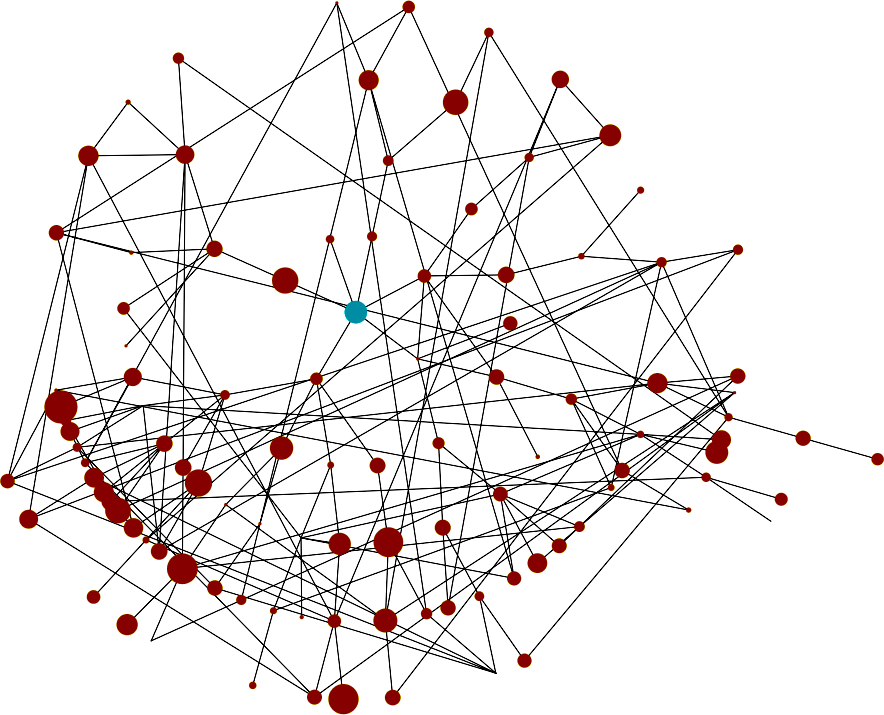
\includegraphics[width=0.6\textwidth]{oriflame7_view1.png}\end{center}
  \end{frame}
  \begin{frame}
    \frametitle{Hlavní výsledky}
    \framesubtitle{Průběh šíření}
    \begin{enumerate}
      \item 
      \item
      \item
    \end{enumerate}
    \begin{center}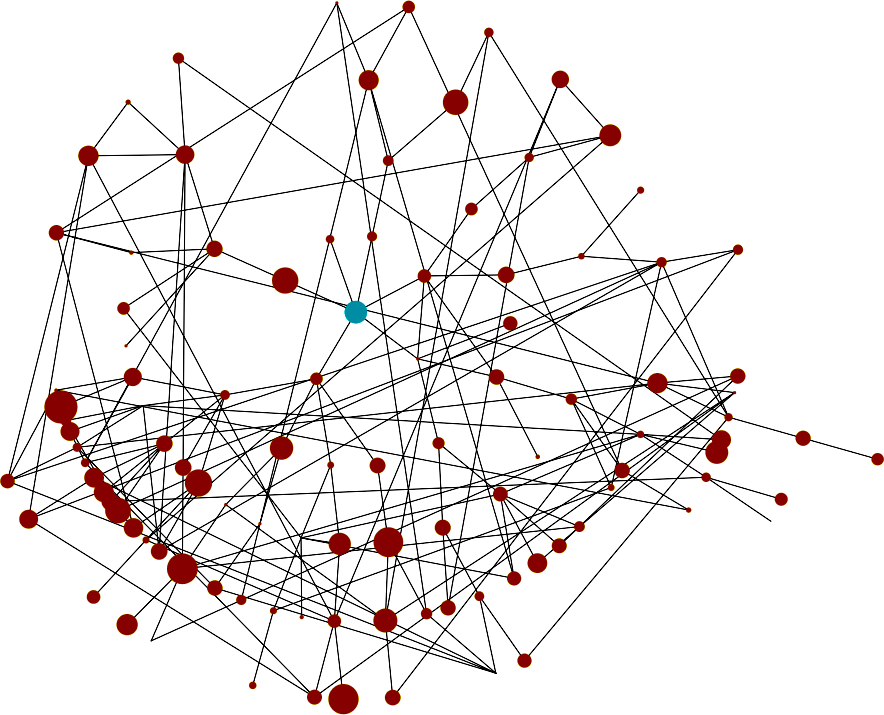
\includegraphics[width=0.6\textwidth]{oriflame7_view1.png}\end{center}
  \end{frame}    
% etc
\end{document}
